\documentclass[11pt]{standalone}
\usepackage{amssymb}
\usepackage{amsmath}
\usepackage[no-math]{fontspec}
\usepackage{unicode-math}
\usepackage{libertinus}
\usepackage{pgf,xcolor}
\usepackage{tikz}
\usetikzlibrary{arrows.meta, backgrounds, calc}
\usepackage{pgfplots}
\pgfplotsset{compat=newest}

\definecolor{my_darkgray}{HTML}{484949}
\definecolor{my_lightgray}{HTML}{F3F4F4}
\definecolor{my_darkblue}{HTML}{005A94}
\definecolor{my_lightblue}{HTML}{CCDEE9}
\definecolor{my_yellow}{HTML}{FFEC7F}
\definecolor{my_red}{HTML}{E60000}
\definecolor{my_orange}{HTML}{E87846}

\begin{document}
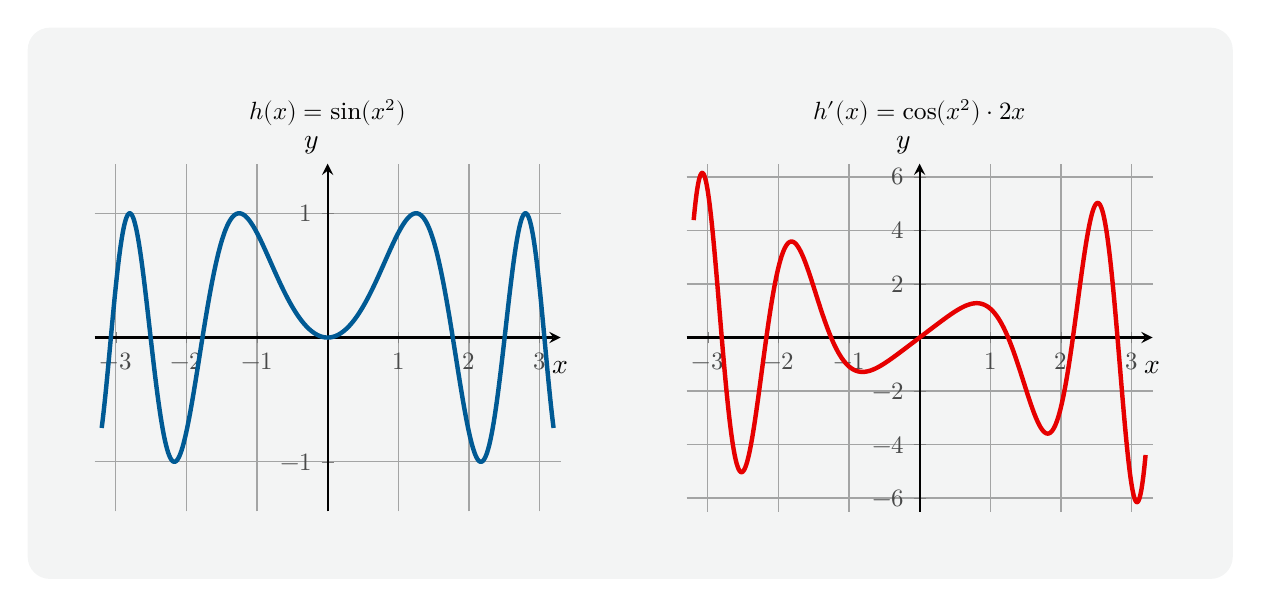
\begin{tikzpicture}[
    show background rectangle,
    background rectangle/.style={fill=my_lightgray, rounded corners=8pt},
    inner frame sep=0.8cm
]

% ── Left plot: h(x) = sin(x²) ──────────────────────────────────────────────
\begin{axis}[
    name=left plot,
    axis lines = center,
    xlabel = {$x$},
    ylabel = {$y$},
    xlabel style = {at={(axis cs:3.3,0)}, anchor=north, yshift=-5pt},
    ylabel style = {anchor=south east},
    title = {$h(x) = \sin(x^2)$},
    title style = {font=\small, yshift=4pt},
    grid = both,
    grid style = {line width=0.3pt, draw=my_darkgray!30},
    major grid style = {line width=0.5pt, draw=my_darkgray!50},
    % axis equal omitted: would compress the oscillations unreadably
    axis line style = {thick},
    xmin = -3.3, xmax = 3.3,
    ymin = -1.4,  ymax = 1.4,
    xtick = {-3,-2,-1,0,1,2,3},
    ytick = {-1,0,1},
    yticklabel style = {
        /pgf/number format/fixed,
        /pgf/number format/precision=1,
        font=\small,
        text=my_darkgray
    },
    xticklabel style = {font=\small, text=my_darkgray},
    width=7.5cm, height=6cm,
    clip=true,
]
\addplot[
    draw=my_darkblue,
    samples=800,
    ultra thick,
    domain=-3.2:3.2
]{ sin(deg(x^2)) };
\end{axis}

% ── Right plot: h'(x) = cos(x²)·2x ────────────────────────────────────────
\begin{axis}[
    name=right plot,
    at={($(left plot.east)+(1.6cm,0)$)},
    anchor=west,
    axis lines = center,
    xlabel = {$x$},
    ylabel = {$y$},
    xlabel style = {at={(axis cs:3.3,0)}, anchor=north, yshift=-5pt},
    ylabel style = {anchor=south east},
    title = {$h'(x) = \cos(x^2)\cdot 2x$},
    title style = {font=\small, yshift=4pt},
    grid = both,
    grid style = {line width=0.3pt, draw=my_darkgray!30},
    major grid style = {line width=0.5pt, draw=my_darkgray!50},
    % axis equal omitted: y range ±6 vs x range ±3 would distort the graph
    axis line style = {thick},
    xmin = -3.3, xmax = 3.3,
    ymin = -6.5,  ymax = 6.5,
    xtick = {-3,-2,-1,0,1,2,3},
    ytick = {-6,-4,-2,0,2,4,6},
    yticklabel style = {
        /pgf/number format/fixed,
        /pgf/number format/precision=0,
        font=\small,
        text=my_darkgray
    },
    xticklabel style = {font=\small, text=my_darkgray},
    width=7.5cm, height=6cm,
    clip=true,
]
\addplot[
    draw=my_red,
    samples=800,
    ultra thick,
    domain=-3.2:3.2
]{ cos(deg(x^2)) * 2*x };
\end{axis}

\end{tikzpicture}
\end{document}
